\documentclass[12pt]{article}
\usepackage[utf8]{inputenc}
\usepackage[utf8]{vietnam}
\usepackage{amsmath, amssymb, amsfonts}
\usepackage{tikz}
\usetikzlibrary{arrows.meta, calc, angles, quotes}
\usepackage{geometry}
\geometry{a4paper, margin=0.8in}
\usepackage{xcolor}
\usepackage{pifont}
\usepackage[most]{tcolorbox}

% Colors
\definecolor{myblue}{RGB}{0, 102, 204}
\definecolor{myred}{RGB}{204, 0, 0}
\definecolor{highlightyellow}{RGB}{255, 235, 59}

% Custom components
\newcommand{\bluecheck}{%
  \tikz[baseline=-0.5ex]\node[circle,fill=myblue,inner sep=0.5pt,minimum size=10pt]{\textcolor{white}{\fontsize{5}{5}\selectfont\checkmark}};%
}
\newcommand{\handwrite}{\textcolor{myblue}{\ding{46}}}

\newtcolorbox{notebox}[1][]{
  colback=myred!5!white,
  colframe=myred,
  arc=4pt,
  boxrule=0.5pt,
  leftrule=3pt,
  #1
}

\begin{document}

% Header
\begin{center}
    \textcolor{myred}{\small thuvienhoclieu.com} \\
    \vspace{0.2cm}
    \colorbox{highlightyellow}{\textbf{\color{myred}{\large\quad CHỦ ĐỀ 8. HÌNH HỌC KHÔNG GIAN\quad}}}
\end{center}

\vspace{0.3cm}

\noindent\textbf{\color{myblue}{\large A. KIẾN THỨC CẦN NHỚ}}\\
\noindent\textbf{\color{myblue}{\large I. QUAN HỆ SONG SONG TRONG KHÔNG GIAN}}\\

\noindent\textbf{\color{myblue}{1. Giao tuyến của 2 mp:}} Đường thẳng $d$ chung của hai mặt phẳng $(P)$ và $(Q)$ được gọi là giao tuyến của $(P)$ và $(Q)$, kí hiệu $d = (P) \cap (Q)$.\\

\noindent\textbf{\color{myblue}{2. Thiết diện:}} Thiết diện của mặt phẳng $\underline{(\alpha)}$ với hình chóp $\underline{(H)}$ là phần chung giữa mặt phẳng $\underline{(\alpha)}$ và hình chóp $\underline{(H)}$.\\

\noindent\textbf{\color{myblue}{3. Vị trí tương đối của hai đường thẳng trong không gian}}\\
\textit{TH1: $a$ và $b$ đồng phẳng}
\begin{itemize}
    \item[\bluecheck] $a$ cắt $b \Leftrightarrow a \cap b = \{M\}$.
    \item[\bluecheck] $a \parallel b \Leftrightarrow a \cap b = \varnothing$.
    \item[\bluecheck] $a \equiv b \Leftrightarrow a \cap b = a$.
\end{itemize}
\textit{TH2: không có mp nào chứa $a$ và $b$, ta nói \textbf{\color{myblue}{$a$ và $b$ chéo nhau}}.}

\vspace{0.4cm}

% 4 Diagrams for relative positions of two lines
\begin{center}
\begin{tabular}{cccc}
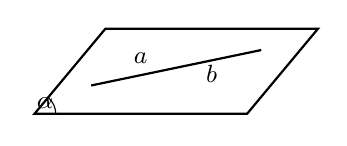
\begin{tikzpicture}[scale=0.9, >=stealth]
  \draw[thick] (0,0) -- (3,0) -- (4,1.2) -- (1,1.2) -- cycle;
  \draw (0.3,0) arc (0:50:0.3);
  \node at (0.15,0.15) {\small $\alpha$};
  \draw[thick] (0.8,0.4) -- (3.2,0.9);
  \node[above] at (1.5,0.57) {\small $a$};
  \node[below] at (2.5,0.82) {\small $b$};
\end{tikzpicture}
&
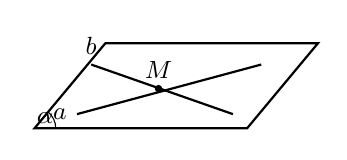
\begin{tikzpicture}[scale=0.9, >=stealth]
  \draw[thick] (0,0) -- (3,0) -- (4,1.2) -- (1,1.2) -- cycle;
  \draw (0.3,0) arc (0:50:0.3);
  \node at (0.15,0.15) {\small $\alpha$};
  \draw[thick] (0.6,0.2) node[left] {\small $a$} -- (3.2,0.9);
  \draw[thick] (0.8,0.9) node[above] {\small $b$} -- (2.8,0.2);
  \coordinate (M) at (1.75,0.56);
  \fill (M) circle (1.5pt);
  \node[above] at (1.75,0.56) {\small $M$};
\end{tikzpicture}
&
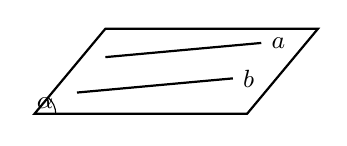
\begin{tikzpicture}[scale=0.9, >=stealth]
  \draw[thick] (0,0) -- (3,0) -- (4,1.2) -- (1,1.2) -- cycle;
  \draw (0.3,0) arc (0:50:0.3);
  \node at (0.15,0.15) {\small $\alpha$};
  \draw[thick] (1.0,0.8) -- (3.2,1.0) node[right] {\small $a$};
  \draw[thick] (0.6,0.3) -- (2.8,0.5) node[right] {\small $b$};
\end{tikzpicture}
&
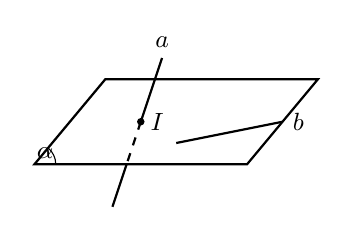
\begin{tikzpicture}[scale=0.9, >=stealth]
  \draw[thick] (0,0) -- (3,0) -- (4,1.2) -- (1,1.2) -- cycle;
  \draw (0.3,0) arc (0:50:0.3);
  \node at (0.15,0.15) {\small $\alpha$};
  \draw[thick] (2.0,0.3) -- (3.5,0.6) node[right] {\small $b$};
  \coordinate (I) at (1.5,0.6);
  \draw[thick] (1.8,1.5) node[above] {\small $a$} -- (I);
  \draw[dashed, thick] (I) -- (1.3,0);
  \draw[thick] (1.3,0) -- (1.1,-0.6);
  \fill (I) circle (1.5pt) node[right] {\small $I$};
\end{tikzpicture}
\\
$a \equiv b$ & $a \cap b = \{M\}$ & $a \parallel b$ & $a, b$ chéo nhau \\
a) & b) & c) & d)
\end{tabular}
\end{center}

\vspace{0.4cm}

\noindent\textbf{\color{myblue}{a/ Hai đường thẳng song song:}} nếu chúng cùng nằm trên một mặt phẳng và không có điểm chung.

\begin{notebox}
\noindent\textbf{\color{myred}{\textit{*Chú ý:}}}\\
\indent 1. Hai đường thẳng gọi là \textit{chéo nhau} nếu chúng không đồng phẳng.\\
\indent 2. Cho hai đường thẳng song song $a$ và $b$. Có duy nhất một mặt phẳng chứa hai đường thẳng đó, kí hiệu $\text{mp}(a, b)$.
\end{notebox}

\vspace{0.2cm}

\noindent\textbf{\color{myblue}{b/ Tính chất cơ bản về hai đường thẳng song song.}}\\
\textbf{+} Nếu ba mp phân biệt đôi một cắt nhau theo ba giao tuyến phân biệt thì ba giao tuyến ấy hoặc đồng quy hoặc đôi một song song với nhau.

\vspace{0.4cm}

% 2 Diagrams for 3 planes intersection
\begin{center}
\begin{tabular}{cc}
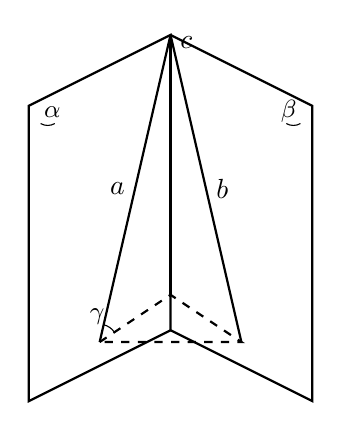
\begin{tikzpicture}[scale=1.5, >=stealth]
  \coordinate (V) at (0,2);
  \coordinate (O) at (0,-0.5);
  \coordinate (TL) at (-1.2, 1.4);
  \coordinate (BL) at (-1.2, -1.1);
  \coordinate (TR) at (1.2, 1.4);
  \coordinate (BR) at (1.2, -1.1);

  \draw[thick] (TL) -- (V) -- (O) -- (BL) -- cycle;
  \draw[thick] (V) -- (TR) -- (BR) -- (O);

  \draw (-1.1, 1.25) arc (240:300:0.12);
  \node at (-1.0, 1.35) {\small $\alpha$};
  
  \draw (1.1, 1.25) arc (300:240:0.12);
  \node at (1.0, 1.35) {\small $\beta$};

  \coordinate (A0) at (-0.6, -0.6);
  \coordinate (B0) at (0.6, -0.6);
  \coordinate (C0) at (0, -0.2);

  \draw[dashed, thick] (A0) -- (C0) -- (B0) -- cycle;

  \draw[thick] (A0) -- (V) node[midway, left] {$a$};
  \draw[thick] (B0) -- (V) node[midway, right] {$b$};
  \draw[thick] (C0) -- (V);
  \node[above right] at (0, 1.8) {$c$};

  \draw (-0.6, -0.6) + (34:0.15) arc (34:77:0.15);
  \node at (-0.62, -0.38) {\small $\gamma$};
\end{tikzpicture}
&
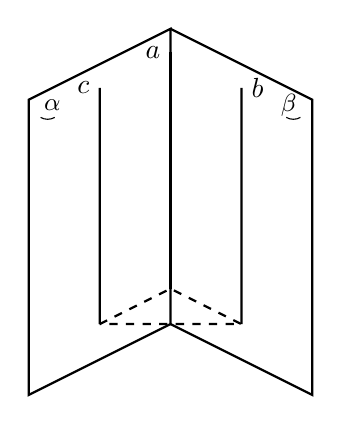
\begin{tikzpicture}[scale=1.5, >=stealth]
  \coordinate (V) at (0,2);
  \coordinate (O) at (0,-0.5);
  \coordinate (TL) at (-1.2, 1.4);
  \coordinate (BL) at (-1.2, -1.1);
  \coordinate (TR) at (1.2, 1.4);
  \coordinate (BR) at (1.2, -1.1);

  \draw[thick] (TL) -- (V) -- (O) -- (BL) -- cycle;
  \draw[thick] (V) -- (TR) -- (BR) -- (O);

  \draw (-1.1, 1.25) arc (240:300:0.12);
  \node at (-1.0, 1.35) {\small $\alpha$};
  
  \draw (1.1, 1.25) arc (300:240:0.12);
  \node at (1.0, 1.35) {\small $\beta$};

  \coordinate (C0) at (-0.6, -0.5);
  \coordinate (B0) at (0.6, -0.5);
  \coordinate (A0) at (0, -0.2);

  \draw[dashed, thick] (C0) -- (A0) -- (B0) -- cycle;

  \draw[thick] (C0) -- (-0.6, 1.5) node[left] {$c$};
  \draw[thick] (B0) -- (0.6, 1.5) node[right] {$b$};
  \draw[thick] (A0) -- (0, 1.8) node[left] {$a$};
\end{tikzpicture}
\end{tabular}
\end{center}

\vspace{0.4cm}

\noindent\textbf{+} Nếu hai mp phân biệt lần lượt chứa hai đt song song thì giao tuyến của chúng (nếu có) cũng song song với hai đt đó hoặc trùng với một trong hai đt đó.

\vspace{0.4cm}

% 3 Diagrams for parallel lines in intersecting planes
\begin{center}
\begin{tabular}{ccc}
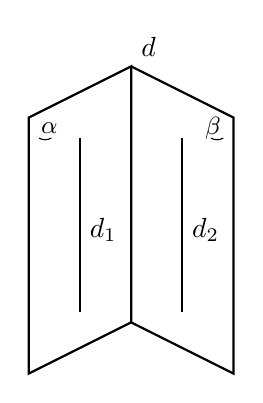
\begin{tikzpicture}[scale=1.3, >=stealth]
  \coordinate (V) at (0,2);
  \coordinate (O) at (0,-0.5);
  \coordinate (TL) at (-1.0, 1.5);
  \coordinate (BL) at (-1.0, -1.0);
  \coordinate (TR) at (1.0, 1.5);
  \coordinate (BR) at (1.0, -1.0);

  \draw[thick] (TL) -- (V) -- (O) -- (BL) -- cycle;
  \draw[thick] (V) -- (TR) -- (BR) -- (O);

  \draw (-0.9, 1.3) arc (240:300:0.12);
  \node at (-0.8, 1.4) {\small $\alpha$};
  \draw (0.9, 1.3) arc (300:240:0.12);
  \node at (0.8, 1.4) {\small $\beta$};

  \draw[thick] (0, -0.5) -- (0, 2) node[above right] {$d$};
  \draw[thick] (-0.5, -0.4) -- (-0.5, 1.3);
  \node[right] at (-0.5, 0.4) {$d_1$};
  \draw[thick] (0.5, -0.4) -- (0.5, 1.3);
  \node[right] at (0.5, 0.4) {$d_2$};
\end{tikzpicture}
&
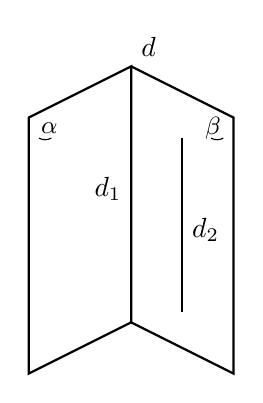
\begin{tikzpicture}[scale=1.3, >=stealth]
  \coordinate (V) at (0,2);
  \coordinate (O) at (0,-0.5);
  \coordinate (TL) at (-1.0, 1.5);
  \coordinate (BL) at (-1.0, -1.0);
  \coordinate (TR) at (1.0, 1.5);
  \coordinate (BR) at (1.0, -1.0);

  \draw[thick] (TL) -- (V) -- (O) -- (BL) -- cycle;
  \draw[thick] (V) -- (TR) -- (BR) -- (O);

  \draw (-0.9, 1.3) arc (240:300:0.12);
  \node at (-0.8, 1.4) {\small $\alpha$};
  \draw (0.9, 1.3) arc (300:240:0.12);
  \node at (0.8, 1.4) {\small $\beta$};

  \draw[thick] (0, -0.5) -- (0, 2) node[above right] {$d$};
  \node[left] at (0, 0.8) {$d_1$};
  \draw[thick] (0.5, -0.4) -- (0.5, 1.3);
  \node[right] at (0.5, 0.4) {$d_2$};
\end{tikzpicture}
&
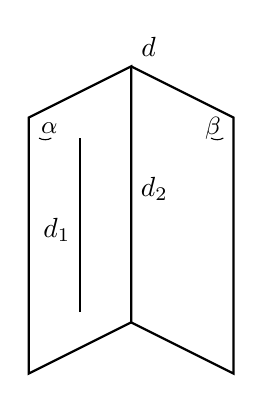
\begin{tikzpicture}[scale=1.3, >=stealth]
  \coordinate (V) at (0,2);
  \coordinate (O) at (0,-0.5);
  \coordinate (TL) at (-1.0, 1.5);
  \coordinate (BL) at (-1.0, -1.0);
  \coordinate (TR) at (1.0, 1.5);
  \coordinate (BR) at (1.0, -1.0);

  \draw[thick] (TL) -- (V) -- (O) -- (BL) -- cycle;
  \draw[thick] (V) -- (TR) -- (BR) -- (O);

  \draw (-0.9, 1.3) arc (240:300:0.12);
  \node at (-0.8, 1.4) {\small $\alpha$};
  \draw (0.9, 1.3) arc (300:240:0.12);
  \node at (0.8, 1.4) {\small $\beta$};

  \draw[thick] (0, -0.5) -- (0, 2) node[above right] {$d$};
  \node[right] at (0, 0.8) {$d_2$};
  \draw[thick] (-0.5, -0.4) -- (-0.5, 1.3);
  \node[left] at (-0.5, 0.4) {$d_1$};
\end{tikzpicture}
\\
a) & b) & c)
\end{tabular}
\end{center}

\vspace{0.4cm}

\noindent\textbf{+} Nếu hai mp phân biệt cùng song song với một đường thẳng thì giao tuyến của chúng (nếu có) cũng song song với đường thẳng đó.

\vspace{0.4cm}

\begin{center}
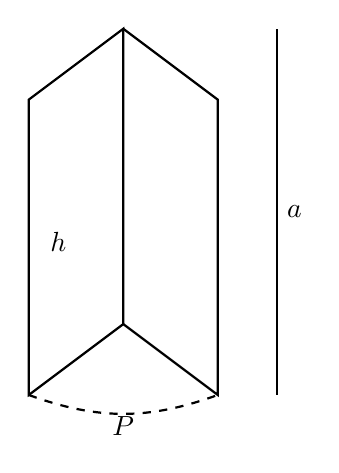
\begin{tikzpicture}[scale=1.5, >=stealth]
  \coordinate (V) at (0,2);
  \coordinate (O) at (0,-0.5);
  \coordinate (TL) at (-0.8, 1.4);
  \coordinate (BL) at (-0.8, -1.1);
  \coordinate (TR) at (0.8, 1.4);
  \coordinate (BR) at (0.8, -1.1);

  \draw[thick] (TL) -- (V) -- (O) -- (BL) -- cycle;
  \draw[thick] (V) -- (TR) -- (BR) -- (O);

  \draw[dashed, thick] (O) -- (V);
  \draw[dashed, thick] (BL) to[out=-20, in=200] (BR);

  \draw[thick] (1.3, -1.1) -- (1.3, 2.0) node[midway, right] {$a$};

  \node[left] at (-0.4, 0.2) {$h$};
  \node[below] at (0, -1.2) {$P$};
\end{tikzpicture}
\end{center}

\newpage

% Page 2: Line & Plane Relative Positions
\noindent\textbf{\color{myblue}{\large 4. Vị trí tương đối của đường thẳng và mặt phẳng}}\\
Cho đường thẳng $a$ và mặt phẳng $(P)$. Khi đó có thể xảy ra một trong ba trường hợp sau:

\noindent\textbf{+ TH 1:} $a$ và $(P)$ có từ hai điểm chung phân biệt trở lên (Hình 2a), suy ra mọi điểm thuộc $a$ đều thuộc $(P)$, ta nói $a$ nằm trong $(P)$, kí hiệu $a \subset (P)$.

\noindent\textbf{+ TH 2:} $a$ và $(P)$ có một điểm chung duy nhất $A$ (Hình 2b), ta nói $a$ cắt $(P)$ tại $A$, kí hiệu $a \cap (P) = \{A\}$.

\noindent\textbf{+ TH 3:} $a$ và $(P)$ không có điểm chung nào (Hình 2c), ta nói $a$ song song với $(P)$, kí hiệu $a \parallel (P)$.

\vspace{0.4cm}

% 3 Diagrams for line & plane relative positions
\begin{center}
\begin{tabular}{ccc}
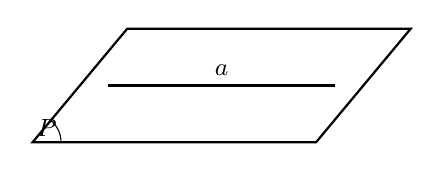
\begin{tikzpicture}[scale=1.2, >=stealth]
  \draw[thick] (0,0) -- (3,0) -- (4,1.2) -- (1,1.2) -- cycle;
  \draw (0.3,0) arc (0:50:0.3);
  \node at (0.15,0.15) {\small $P$};
  \draw[thick] (0.8, 0.6) -- (3.2, 0.6);
  \node[above] at (2.0, 0.6) {\small $a$};
\end{tikzpicture}
&
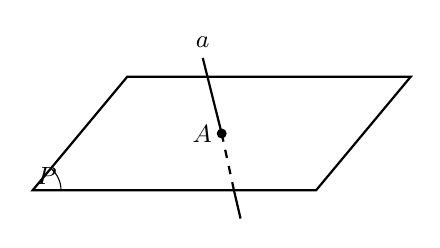
\begin{tikzpicture}[scale=1.2, >=stealth]
  \draw[thick] (0,0) -- (3,0) -- (4,1.2) -- (1,1.2) -- cycle;
  \draw (0.3,0) arc (0:50:0.3);
  \node at (0.15,0.15) {\small $P$};
  
  \coordinate (A) at (2.0, 0.6);
  \draw[thick] (1.8, 1.4) node[above] {\small $a$} -- (A);
  \draw[dashed, thick] (A) -- (2.13, 0);
  \draw[thick] (2.13, 0) -- (2.2, -0.3);
  
  \fill (A) circle (1.5pt) node[left] {\small $A$};
\end{tikzpicture}
&
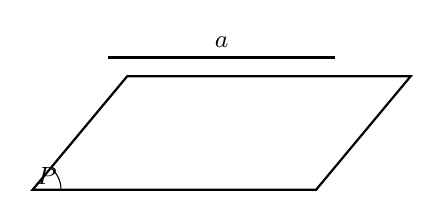
\begin{tikzpicture}[scale=1.2, >=stealth]
  \draw[thick] (0,0) -- (3,0) -- (4,1.2) -- (1,1.2) -- cycle;
  \draw (0.3,0) arc (0:50:0.3);
  \node at (0.15,0.15) {\small $P$};
  \draw[thick] (0.8, 1.4) -- (3.2, 1.4);
  \node[above] at (2.0, 1.4) {\small $a$};
\end{tikzpicture}
\\
Hình 2a & Hình 2b & Hình 2c
\end{tabular}
\end{center}

\vspace{0.4cm}

\noindent\textbf{\color{myblue}{a/ Đường thẳng song song mặt phẳng:}} $a \parallel (P)$ nếu chúng không có điểm chung.

\noindent\textbf{\color{myblue}{b/ Điều kiện để một đường thẳng song song với 1 mặt phẳng}}\\
\textbf{+} Nếu đường thẳng $d$ không nằm trong mặt phẳng $(\alpha)$ và $d$ song song với đường thẳng $d'$ nằm trong $(\alpha)$ thì $d$ song song với $(\alpha)$.

\vspace{0.3cm}

\begin{center}
\begin{minipage}{0.45\textwidth}
\[
\begin{cases}
d \not\subset (\alpha) \\
d \parallel d' \\
d' \subset (\alpha)
\end{cases}
\Rightarrow d \parallel (\alpha)
\]
\end{minipage}
\hfill
\begin{minipage}{0.45\textwidth}
\begin{center}
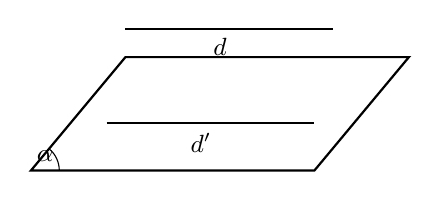
\begin{tikzpicture}[scale=1.2, >=stealth]
  \draw[thick] (0,0) -- (3,0) -- (4,1.2) -- (1,1.2) -- cycle;
  \draw (0.3,0) arc (0:50:0.3);
  \node at (0.15,0.15) {\small $\alpha$};
  \draw[thick] (0.8, 0.5) -- (3.0, 0.5);
  \node[below] at (1.8, 0.5) {\small $d'$};
  \draw[thick] (1.0, 1.5) -- (3.2, 1.5);
  \node[below] at (2.0, 1.5) {\small $d$};
\end{tikzpicture}
\end{center}
\end{minipage}
\end{center}

\vspace{0.4cm}

\noindent\textbf{\color{myblue}{c/ Tính chất cơ bản của đường thẳng và mặt phẳng song song}}\\
\textbf{+} Cho đường thẳng $d$ song song với mặt phẳng $(\alpha)$. Nếu mặt phẳng $(\beta)$ đi qua $d$ và cắt $(\alpha)$ theo giao tuyến $d'$ thì $d' \parallel d$.

\vspace{0.3cm}

\begin{center}
\begin{minipage}{0.45\textwidth}
\[
\begin{cases}
d \parallel (\alpha) \\
d \subset (\beta) \\
(\alpha) \cap (\beta) = d'
\end{cases}
\Rightarrow d' \parallel d
\]
\end{minipage}
\hfill
\begin{minipage}{0.45\textwidth}
\begin{center}
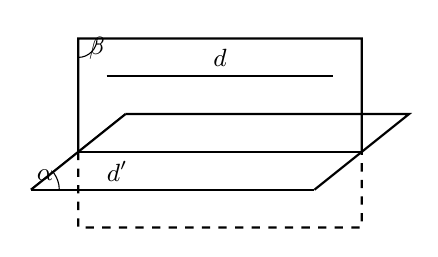
\begin{tikzpicture}[scale=1.2, >=stealth]
  \coordinate (A_TL) at (1.0, 0.4);
  \coordinate (A_TR) at (4.0, 0.4);
  \coordinate (A_BR) at (3.0, -0.4);
  \coordinate (A_BL) at (0, -0.4);
  
  \draw[thick] (A_TL) -- (A_TR) -- (A_BR);
  \draw[thick] (A_BL) -- (A_TL);
  
  \coordinate (B_BL) at (0.5, -0.8);
  \coordinate (B_BR) at (3.5, -0.8);
  \coordinate (B_TL) at (0.5, 1.2);
  \coordinate (B_TR) at (3.5, 1.2);
  
  \draw[thick] (0.5, 0) -- (B_TL) -- (B_TR) -- (3.5, 0);
  \draw[dashed, thick] (0.5, 0) -- (B_BL) -- (B_BR) -- (3.5, 0);
  \draw[thick] (A_BR) -- (A_BL);
  
  \draw (0.3, -0.4) arc (0:38:0.3);
  \node at (0.15, -0.25) {\small $\alpha$};
  
  \draw (0.5, 1.0) arc (-90:0:0.2);
  \node at (0.7, 1.1) {\small $\beta$};
  
  \draw[thick] (0.8, 0.8) -- (3.2, 0.8);
  \node[above] at (2.0, 0.8) {\small $d$};
  
  \draw[thick] (0.5, 0) -- (3.5, 0);
  \node[below right] at (0.7, 0) {\small $d'$};
\end{tikzpicture}
\end{center}
\end{minipage}
\end{center}

\vspace{0.4cm}

\noindent\textbf{+} Nếu hai mặt phẳng phân biệt cùng song song với một đường thẳng thì giao tuyến của chúng (nếu có) cũng song song với đường thẳng đó.

\vspace{0.4cm}

\begin{center}
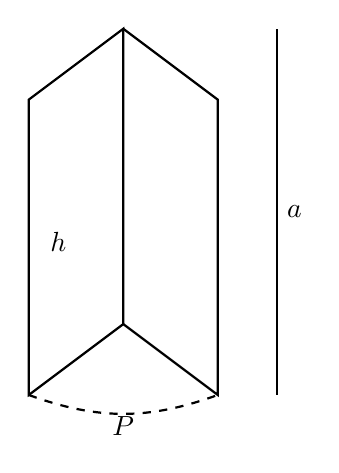
\begin{tikzpicture}[scale=1.5, >=stealth]
  \coordinate (V) at (0,2);
  \coordinate (O) at (0,-0.5);
  \coordinate (TL) at (-0.8, 1.4);
  \coordinate (BL) at (-0.8, -1.1);
  \coordinate (TR) at (0.8, 1.4);
  \coordinate (BR) at (0.8, -1.1);

  \draw[thick] (TL) -- (V) -- (O) -- (BL) -- cycle;
  \draw[thick] (V) -- (TR) -- (BR) -- (O);

  \draw[dashed, thick] (O) -- (V);
  \draw[dashed, thick] (BL) to[out=-20, in=200] (BR);

  \draw[thick] (1.3, -1.1) -- (1.3, 2.0) node[midway, right] {$a$};

  \node[left] at (-0.4, 0.2) {$h$};
  \node[below] at (0, -1.2) {$P$};
\end{tikzpicture}
\end{center}

\newpage

% Page 3: Two Planes Relative Positions
\noindent\textbf{\color{myblue}{\large 5. Vị trí tương đối giữa 2 mặt phẳng $(\alpha)$ và $(\beta)$ có 3 vị trí tương đối}}\\

\noindent\textbf{+ TH 1:} $(P)$ và $(Q)$ có ba điểm chung không thẳng hàng, ta nói hai mặt phẳng $(P)$ và $(Q)$ trùng nhau, kí hiệu $(P) \equiv (Q)$.

\vspace{0.2cm}
\begin{center}
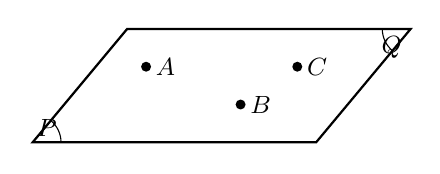
\begin{tikzpicture}[scale=1.2, >=stealth]
  \draw[thick] (0,0) -- (3,0) -- (4,1.2) -- (1,1.2) -- cycle;
  \draw (0.3,0) arc (0:50:0.3);
  \node at (0.15,0.15) {\small $P$};
  \draw (4,1.2) + (180:0.3) arc (180:230:0.3);
  \node at (3.8,1.0) {\small $Q$};
  
  \coordinate (A) at (1.2, 0.8);
  \coordinate (B) at (2.2, 0.4);
  \coordinate (C) at (2.8, 0.8);
  
  \fill (A) circle (1.5pt) node[right] {\small $A$};
  \fill (B) circle (1.5pt) node[right] {\small $B$};
  \fill (C) circle (1.5pt) node[right] {\small $C$};
\end{tikzpicture}
\end{center}

\noindent\textbf{+ TH 2:} $(P)$ và $(Q)$ phân biệt và có một điểm chung, ta nói $(P)$ và $(Q)$ cắt nhau theo giao tuyến $d$ đi qua điểm chung, kí hiệu $(P) \cap (Q) = d$.

\vspace{0.2cm}
\begin{center}
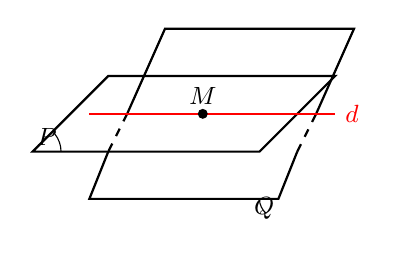
\begin{tikzpicture}[scale=1.2, >=stealth]
  \coordinate (P_BL) at (0, -0.4);
  \coordinate (P_BR) at (2.4, -0.4);
  \coordinate (P_TR) at (3.2, 0.4);
  \coordinate (P_TL) at (0.8, 0.4);
  
  \draw[thick] (P_BL) -- (P_BR) -- (P_TR) -- (P_TL) -- cycle;
  
  \coordinate (Q_TL) at (1.4, 0.9);
  \coordinate (Q_TR) at (3.4, 0.9);
  \coordinate (Q_BL) at (0.6, -0.9);
  \coordinate (Q_BR) at (2.6, -0.9);
  
  \draw[thick] (1.0, 0) -- (Q_TL) -- (Q_TR) -- (3.0, 0);
  
  \draw[dashed, thick] (1.0, 0) -- (0.8, -0.4);
  \draw[thick] (0.8, -0.4) -- (Q_BL) -- (Q_BR) -- (2.8, -0.4);
  \draw[dashed, thick] (2.8, -0.4) -- (3.0, 0);
  
  \draw[thick, red] (0.6, 0) -- (3.2, 0) node[right] {\small $d$};
  
  \coordinate (M) at (1.8, 0);
  \fill (M) circle (1.5pt) node[above] {\small $M$};
  
  \draw (0.3, -0.4) arc (0:38:0.3);
  \node at (0.15, -0.25) {\small $P$};
  
  \draw (2.6, -0.9) + (180:0.2) arc (180:230:0.2);
  \node at (2.45, -1.0) {\small $Q$};
\end{tikzpicture}
\end{center}

\noindent\textbf{+ TH 3:} $(P)$ và $(Q)$ không có bất kì điểm chung nào, nghĩa là $(P) \cap (Q) = \varnothing$, ta nói $(P)$ và $(Q)$ song song với nhau, kí hiệu $(P) \parallel (Q)$ hoặc $(Q) \parallel (P)$.

\vspace{0.2cm}
\begin{center}
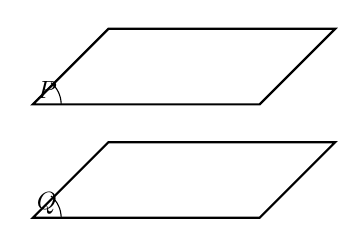
\begin{tikzpicture}[scale=1.2, >=stealth]
  \draw[thick] (0, 0.8) -- (2.4, 0.8) -- (3.2, 1.6) -- (0.8, 1.6) -- cycle;
  \draw (0.3, 0.8) arc (0:50:0.3);
  \node at (0.15, 0.95) {\small $P$};

  \draw[thick] (0, -0.4) -- (2.4, -0.4) -- (3.2, 0.4) -- (0.8, 0.4) -- cycle;
  \draw (0.3, -0.4) arc (0:50:0.3);
  \node at (0.15, -0.25) {\small $Q$};
\end{tikzpicture}
\end{center}

\vspace{0.4cm}

\noindent\textbf{\color{myblue}{a/ Hai mặt phẳng song song:}} $(\alpha)$ và $(\beta)$ được gọi là song song với nhau nếu chúng không có điểm chung.

\begin{notebox}
\noindent\textbf{\color{myred}{\textit{*Chú ý:}}}\\
\indent $(\alpha) \parallel (\beta), d \subset (\alpha) \Rightarrow d \parallel (\beta)$
\end{notebox}

\vspace{0.2cm}

\noindent\textbf{\color{myblue}{b/ Điều kiện để hai mặt phẳng song song}}\\
\textbf{+} Nếu mặt phẳng $(P)$ chứa hai đường thẳng cắt nhau $a, b$ và $a, b$ cùng song song với mặt phẳng $(Q)$ thì $(P)$ song song với $(Q)$.

\vspace{0.2cm}
\begin{center}
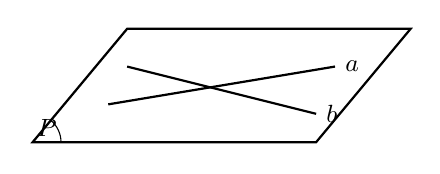
\begin{tikzpicture}[scale=1.2, >=stealth]
  \draw[thick] (0, 0) -- (3, 0) -- (4, 1.2) -- (1, 1.2) -- cycle;
  \draw (0.3, 0) arc (0:50:0.3);
  \node at (0.15, 0.15) {\small $P$};
  
  \draw[thick] (0.8, 0.4) -- (3.2, 0.8) node[right] {\small $a$};
  \draw[thick] (1.0, 0.8) -- (3.0, 0.3) node[right] {\small $b$};
\end{tikzpicture}
\end{center}

\noindent\textbf{+} Nếu mặt phẳng $(\alpha)$ chứa hai đường thẳng cắt nhau $a, b$ và $a, b$ lần lượt song song với hai đường thẳng $a', b'$ nằm trong mặt phẳng $(\beta)$ thì mặt phẳng $(\alpha)$ song song với mặt phẳng $(\beta)$.

\vspace{0.3cm}
\begin{center}
\begin{minipage}{0.45\textwidth}
\[
\begin{cases}
a, b \subset (\alpha) \\
a \cap b = \{O\} \\
a \parallel a', b \parallel b' \\
a', b' \subset (\beta)
\end{cases}
\Rightarrow (\alpha) \parallel (\beta)
\]
\end{minipage}
\hfill
\begin{minipage}{0.45\textwidth}
\begin{center}
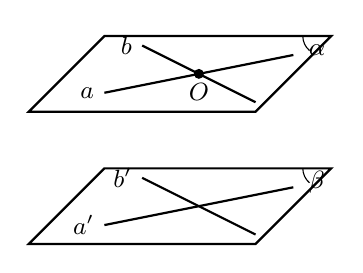
\begin{tikzpicture}[scale=1.2, >=stealth]
  % Plane alpha (top)
  \draw[thick] (0, 0.9) -- (2.4, 0.9) -- (3.2, 1.7) -- (0.8, 1.7) -- cycle;
  \draw (2.9, 1.7) arc (180:230:0.2);
  \node at (3.05, 1.55) {\small $\alpha$};
  
  \coordinate (O) at (1.8, 1.3);
  \draw[thick] (0.8, 1.1) node[left] {\small $a$} -- (2.8, 1.5);
  \draw[thick] (1.2, 1.6) node[left] {\small $b$} -- (2.4, 1.0);
  \fill (O) circle (1.5pt) node[below] {\small $O$};

  % Plane beta (bottom)
  \draw[thick] (0, -0.5) -- (2.4, -0.5) -- (3.2, 0.3) -- (0.8, 0.3) -- cycle;
  \draw (2.9, 0.3) arc (180:230:0.2);
  \node at (3.05, 0.15) {\small $\beta$};
  
  \draw[thick] (0.8, -0.3) node[left] {\small $a'$} -- (2.8, 0.1);
  \draw[thick] (1.2, 0.2) node[left] {\small $b'$} -- (2.4, -0.4);
\end{tikzpicture}
\end{center}
\end{minipage}
\end{center}

\begin{notebox}
\noindent\textbf{\color{myred}{\textit{*Lưu ý:}}}\\
\indent Nếu hai mặt phẳng song song với nhau thì mọi đường thẳng nằm trong mặt phẳng này đều song song với mặt phẳng kia.
\end{notebox}

\vspace{0.2cm}

\noindent\textbf{\color{myblue}{c/ Tính chất của hai mặt phẳng song song}}\\
\textbf{+} Cho hai mặt phẳng $(P)$ và $(Q)$ song song với nhau. Nếu $(R)$ cắt $(P)$ thì cắt $(Q)$ và hai giao tuyến của chúng song song với nhau.

\vspace{0.3cm}
\begin{center}
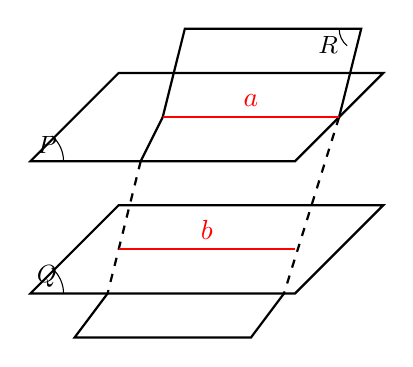
\begin{tikzpicture}[scale=1.4, >=stealth]
  % Draw Q first
  \coordinate (Q_BL) at (0, -0.8);
  \coordinate (Q_BR) at (2.4, -0.8);
  \coordinate (Q_TR) at (3.2, 0);
  \coordinate (Q_TL) at (0.8, 0);
  \draw[thick] (Q_BL) -- (Q_BR) -- (Q_TR) -- (Q_TL) -- cycle;
  \draw (0.3, -0.8) arc (0:50:0.3);
  \node at (0.15, -0.65) {\small $Q$};

  % Draw P
  \coordinate (P_BL) at (0, 0.4);
  \coordinate (P_BR) at (2.4, 0.4);
  \coordinate (P_TR) at (3.2, 1.2);
  \coordinate (P_TL) at (0.8, 1.2);
  \draw[thick] (P_BL) -- (P_BR) -- (P_TR) -- (P_TL) -- cycle;
  \draw (0.3, 0.4) arc (0:50:0.3);
  \node at (0.15, 0.55) {\small $P$};

  % Coordinates for R
  \coordinate (R_TL) at (1.4, 1.6);
  \coordinate (R_TR) at (3.0, 1.6);
  \coordinate (R_BL) at (0.4, -1.2);
  \coordinate (R_BR) at (2.0, -1.2);

  % Draw R
  % Part above P
  \draw[thick] (1.2, 0.8) -- (R_TL) -- (R_TR) -- (2.8, 0.8);
  % Left and Right edges of R (solid/dashed transitions)
  \draw[thick] (1.2, 0.8) -- (1.0, 0.4); 
  \draw[dashed, thick] (1.0, 0.4) -- (0.7, -0.8);
  \draw[thick] (0.7, -0.8) -- (R_BL) -- (R_BR) -- (2.3, -0.8);
  \draw[dashed, thick] (2.8, 0.8) -- (2.3, -0.8);
  
  % Intersection lines a and b
  \draw[thick, red] (1.2, 0.8) -- (2.8, 0.8) node[midway, above] {$a$};
  \draw[thick, red] (0.8, -0.4) -- (2.4, -0.4) node[midway, above] {$b$};

  % Label R
  \draw (R_TR) + (180:0.2) arc (180:230:0.2);
  \node at (2.7, 1.45) {\small $R$};
\end{tikzpicture}
\end{center}

\noindent\textbf{+} Ba mặt phẳng đôi một song song chắn trên hai cát tuyến bất kì những đoạn thẳng tương ứng tỉ lệ:
\[
\frac{AB}{A'B'} = \frac{BC}{B'C'} = \frac{CA}{C'A'}
\]

\vspace{0.4cm}
% Diagram for Thales Theorem
\begin{center}
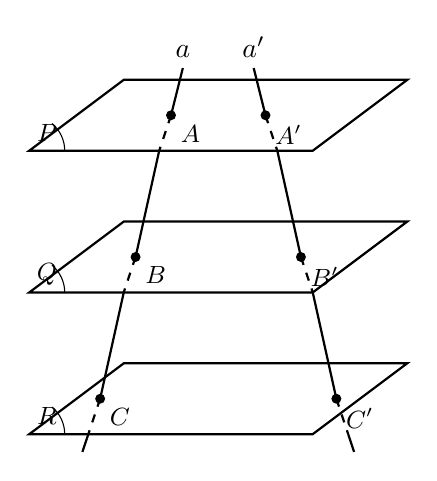
\begin{tikzpicture}[scale=1.5, >=stealth]
  % Plane P (top)
  \draw[thick] (0, 1.2) -- (2.4, 1.2) -- (3.2, 1.8) -- (0.8, 1.8) -- cycle;
  \draw (0.3, 1.2) arc (0:50:0.3);
  \node at (0.15, 1.35) {\small $P$};

  % Plane Q (middle)
  \draw[thick] (0, 0.0) -- (2.4, 0.0) -- (3.2, 0.6) -- (0.8, 0.6) -- cycle;
  \draw (0.3, 0.0) arc (0:50:0.3);
  \node at (0.15, 0.15) {\small $Q$};

  % Plane R (bottom)
  \draw[thick] (0, -1.2) -- (2.4, -1.2) -- (3.2, -0.6) -- (0.8, -0.6) -- cycle;
  \draw (0.3, -1.2) arc (0:50:0.3);
  \node at (0.15, -1.05) {\small $R$};

  % Transversal line a
  \draw[thick] (1.3, 1.9) node[above] {$a$} -- (1.2, 1.5);
  \draw[dashed, thick] (1.2, 1.5) -- (1.1, 1.2);
  \draw[thick] (1.1, 1.2) -- (0.9, 0.3);
  \draw[dashed, thick] (0.9, 0.3) -- (0.8, 0.0);
  \draw[thick] (0.8, 0.0) -- (0.6, -0.9);
  \draw[dashed, thick] (0.6, -0.9) -- (0.5, -1.2);
  \draw[thick] (0.5, -1.2) -- (0.45, -1.35);

  % Transversal line a'
  \draw[thick] (1.9, 1.9) node[above] {$a'$} -- (2.0, 1.5);
  \draw[dashed, thick] (2.0, 1.5) -- (2.1, 1.2);
  \draw[thick] (2.1, 1.2) -- (2.3, 0.3);
  \draw[dashed, thick] (2.3, 0.3) -- (2.4, 0.0);
  \draw[thick] (2.4, 0.0) -- (2.6, -0.9);
  \draw[dashed, thick] (2.6, -0.9) -- (2.7, -1.2);
  \draw[thick] (2.7, -1.2) -- (2.75, -1.35);

  % Fill intersection points
  \fill (1.2, 1.5) circle (1.2pt) node[below right] {\small $A$};
  \fill (0.9, 0.3) circle (1.2pt) node[below right] {\small $B$};
  \fill (0.6, -0.9) circle (1.2pt) node[below right] {\small $C$};

  \fill (2.0, 1.5) circle (1.2pt) node[below right] {\small $A'$};
  \fill (2.3, 0.3) circle (1.2pt) node[below right] {\small $B'$};
  \fill (2.6, -0.9) circle (1.2pt) node[below right] {\small $C'$};
\end{tikzpicture}
\end{center}

\newpage

% Page 4: Prisms, Projection & Perpendiculars
\noindent\textbf{\color{myblue}{d/ Hình lăng trụ và hình hộp}}\\

% 3 Diagrams of Prisms side-by-side
\begin{center}
\begin{tabular}{ccc}
\begin{tikzpicture}[scale=1.1, >=stealth]
  \coordinate (A2) at (0, 0);
  \coordinate (B2) at (1.0, -0.2);
  \coordinate (C2) at (0.4, 0.4);
  \coordinate (A1) at (0.2, 1.5);
  \coordinate (B1) at (1.2, 1.3);
  \coordinate (C1) at (0.6, 1.9);

  \draw[thick] (A2) -- (B2);
  \draw[dashed, thick] (B2) -- (C2) -- (A2);
  \draw[thick] (A1) -- (A2);
  \draw[thick] (B1) -- (B2);
  \draw[dashed, thick] (C1) -- (C2);
  \draw[thick] (A1) -- (B1) -- (C1) -- cycle;
  
  \node[below, align=center] at (0.6, -0.4) {\small Lăng trụ\\ \small tam giác};
\end{tikzpicture}
&
\begin{tikzpicture}[scale=1.1, >=stealth]
  \coordinate (A2) at (0, 0);
  \coordinate (B2) at (1.0, -0.2);
  \coordinate (C2) at (1.5, 0.3);
  \coordinate (D2) at (0.5, 0.5);
  \coordinate (A1) at (0.2, 1.5);
  \coordinate (B1) at (1.2, 1.3);
  \coordinate (C1) at (1.7, 1.8);
  \coordinate (D1) at (0.7, 2.0);

  \draw[thick] (A2) -- (B2) -- (C2);
  \draw[dashed, thick] (C2) -- (D2) -- (A2);
  \draw[thick] (A1) -- (A2);
  \draw[thick] (B1) -- (B2);
  \draw[thick] (C1) -- (C2);
  \draw[dashed, thick] (D1) -- (D2);
  \draw[thick] (A1) -- (B1) -- (C1) -- (D1) -- cycle;
  
  \node[below, align=center] at (0.85, -0.4) {\small Lăng trụ\\ \small tứ giác};
\end{tikzpicture}
&
\begin{tikzpicture}[scale=1.1, >=stealth]
  \coordinate (A2) at (0.6, -0.3);
  \coordinate (B2) at (0, 0);
  \coordinate (C2) at (0.3, 0.5);
  \coordinate (D2) at (1.0, 0.5);
  \coordinate (E2) at (1.3, 0);
  \coordinate (A1) at (0.8, 1.2);
  \coordinate (B1) at (0.2, 1.5);
  \coordinate (C1) at (0.5, 2.0);
  \coordinate (D1) at (1.2, 2.0);
  \coordinate (E1) at (1.5, 1.5);

  \draw[thick] (B2) -- (A2) -- (E2);
  \draw[dashed, thick] (E2) -- (D2) -- (C2) -- (B2);
  \draw[thick] (A1) -- (A2);
  \draw[thick] (B1) -- (B2);
  \draw[thick] (E1) -- (E2);
  \draw[dashed, thick] (C1) -- (C2);
  \draw[dashed, thick] (D1) -- (D2);
  \draw[thick] (A1) -- (B1) -- (C1) -- (D1) -- E1 -- cycle;

  \node[below, align=center] at (0.75, -0.4) {\small Lăng trụ\\ \small ngũ giác};
\end{tikzpicture}
\end{tabular}
\end{center}

\vspace{0.4cm}

\noindent\textbf{\color{myblue}{6/ Phép chiếu song song}}\\
\textbf{\color{myred}{Hình biểu diễn của một số hình không gian trên mặt phẳng:}}\\
\textbf{+} Hình biểu diễn của một đường tròn thường là một elip.\\
\textbf{+} Hình biểu diễn của một tam giác (vuông, cân, đều) là một tam giác.\\
\textbf{+} Hình biểu diễn của hình vuông, hình chữ nhật, hình thoi, hình bình hành là hình bình hành.\\

\noindent\textbf{\color{myblue}{\large II. QUAN HỆ VUÔNG GÓC TRONG KHÔNG GIAN}}\\
\noindent\textbf{\color{myblue}{1. Hai đường thẳng vuông góc}}\\
Hai đường thẳng $a$ và $b$ được gọi là vuông góc với nhau nếu góc giữa chúng bằng $90^\circ$, kí hiệu $a \perp b$.\\

\noindent\textbf{\color{myblue}{2. Đường thẳng vuông góc với mặt phẳng}}\\
\textbf{a) Định nghĩa}\\
\begin{minipage}{0.5\textwidth}
Đường thẳng $d$ được gọi là vuông góc với mặt phẳng $(P)$ nếu đường thẳng $d$ vuông góc với mọi đường thẳng trong mặt phẳng $(P)$ (Hình 1), kí hiệu $d \perp (P)$ hoặc $(P) \perp d$.
\end{minipage}
\hfill
\begin{minipage}{0.45\textwidth}
\begin{center}
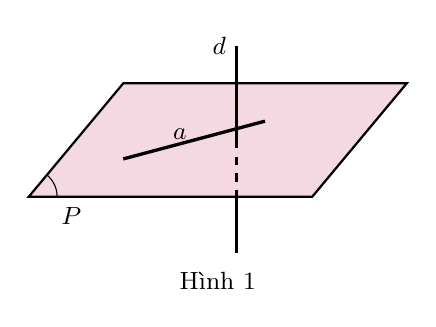
\begin{tikzpicture}[scale=1.2, >=stealth]
  \fill[purple!15] (0,0) -- (3,0) -- (4,1.2) -- (1,1.2) -- cycle;
  \draw[thick] (0,0) -- (3,0) -- (4,1.2) -- (1,1.2) -- cycle;
  \draw (0.3,0) arc (0:50:0.3);
  \node at (0.45,-0.2) {\small $P$};
  
  \draw[very thick] (1.0, 0.4) -- (2.5, 0.8);
  \node[above] at (1.6, 0.5) {\small $a$};
  
  \draw[very thick] (2.2, 1.6) node[left] {\small $d$} -- (2.2, 0.6);
  \draw[dashed, very thick] (2.2, 0.6) -- (2.2, 0.0);
  \draw[very thick] (2.2, 0.0) -- (2.2, -0.6);
  
  \node[below] at (2.0, -0.7) {\small Hình 1};
\end{tikzpicture}
\end{center}
\end{minipage}

\vspace{0.4cm}

\noindent\textbf{\color{myblue}{b) Dấu hiệu nhận biết}}\\
Nếu một đường thẳng vuông góc với hai đường thẳng cắt nhau cùng thuộc một mặt phẳng thì nó vuông góc với mặt phẳng ấy.\\

\noindent\textbf{\color{myblue}{c) Tính chất}}
\begin{itemize}
    \item[\bluecheck] Có duy nhất một mặt phẳng đi qua một điểm cho trước và vuông góc với một đường thẳng cho trước.
    \item[\bluecheck] Có duy nhất một đường thẳng đi qua một điểm cho trước và vuông góc với một mặt phẳng cho trước.
    \item[\bluecheck] Cho hai đường thẳng song song. Một mặt phẳng vuông góc với đường thẳng này thì cũng vuông góc với đường thẳng kia.
    \item[\bluecheck] Hai đường thẳng phân biệt cùng vuông góc với một mặt phẳng thì song song với nhau.
    \item[\bluecheck] Cho hai mặt phẳng song song. Một đường thẳng vuông góc với mặt phẳng này thì cũng vuông góc với mặt phẳng kia.
    \item[\bluecheck] Hai mặt phẳng phân biệt cùng vuông góc với một đường thẳng thì song song với nhau.
\end{itemize}

\newpage

% Page 5: Three Perpendiculars, 2 Planes Perpendicular & Angles
\noindent\textbf{\color{myblue}{d) Định lí ba đường vuông góc}}\\
\begin{minipage}{0.5\textwidth}
Cho đường thẳng $a$ không vuông góc với mặt phẳng $(P)$ và đường thẳng $d$ nằm trong mặt phẳng $(P)$. Khi đó, $d$ vuông góc với $a$ khi và chỉ khi $d$ vuông góc với hình chiếu vuông góc $a'$ của $a$ trên $(P)$ (Hình 2).
\end{minipage}
\hfill
\begin{minipage}{0.45\textwidth}
\begin{center}
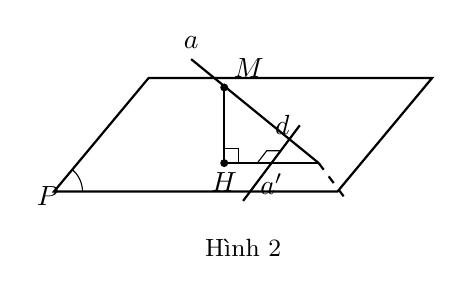
\begin{tikzpicture}[scale=1.2, >=stealth]
  % Plane P
  \draw[thick] (0,0) -- (3,0) -- (4,1.2) -- (1,1.2) -- cycle;
  \draw (0.3,0) arc (0:50:0.3);
  \node at (0.15,0.15) [below left] {$P$};
  
  % Coordinates
  \coordinate (O) at (2.8, 0.3);
  \coordinate (M) at (1.8, 1.1);
  \coordinate (H) at (1.8, 0.3);
  
  % Line a (solid above, dashed below)
  \draw[thick] (1.45, 1.4) node[above] {$a$} -- (O);
  \draw[dashed, thick] (O) -- (3.1, -0.1);
  
  % Vertical line MH
  \draw[thick] (M) -- (H);
  
  % Projection line a' (HO)
  \draw[thick] (H) -- (O) node[midway, below] {$a'$};
  
  % Line d in plane
  \coordinate (D_start) at (2.0, -0.1);
  \coordinate (D_end) at (2.6, 0.7);
  \draw[thick] (D_start) -- (D_end) node[left] {$d$};
  
  % Point labels
  \fill (M) circle (1.2pt) node[above right] {$M$};
  \fill (H) circle (1.2pt) node[below] {$H$};
  
  % Right angle at H
  \draw (1.8, 0.45) -- (1.95, 0.45) -- (1.95, 0.3);
  
  % Right angle between d and HO in perspective
  \draw (2.15, 0.3) -- (2.25, 0.43) -- (2.4, 0.43);
  
  \node[below] at (2.0, -0.4) {\small Hình 2};
\end{tikzpicture}
\end{center}
\end{minipage}

\vspace{0.4cm}

\noindent\textbf{\color{myblue}{3. Hai mặt phẳng vuông góc}}\\
\noindent\textbf{a) Định nghĩa}\\
Hai mặt phẳng $(P)$, $(Q)$ cắt nhau tạo nên bốn góc nhị diện. Nếu một trong các góc nhị diện đó là góc nhị diện vuông thì hai mặt phẳng $(P)$, $(Q)$ gọi là vuông góc với nhau, kí hiệu $(P) \perp (Q)$.\\

\noindent\textbf{b) Dấu hiệu nhận biết}\\
Nếu một mặt phẳng này chứa một đường thẳng mà đường thẳng đó vuông góc với mặt phẳng kia thì hai mặt phẳng đó vuông góc với nhau.\\

\noindent\textbf{c) Tính chất}
\begin{itemize}
    \item[\bluecheck] Nếu hai mặt phẳng vuông góc với nhau thì bất cứ đường thẳng nào nằm trong mặt phẳng này và vuông góc với giao tuyến cũng vuông góc với mặt phẳng kia.
    \item[\bluecheck] Nếu hai mặt phẳng cắt nhau và cùng vuông góc với mặt phẳng thứ ba thì giao tuyến của chúng vuông góc với mặt phẳng thứ ba đó.
\end{itemize}

\vspace{0.4cm}

\noindent\textbf{\color{myblue}{\large II. GÓC TRONG KHÔNG GIAN}}\\
\noindent\textbf{\color{myblue}{1. Góc giữa hai đường thẳng trong không gian}}\\
\begin{minipage}{0.5\textwidth}
Góc giữa hai đường thẳng $a$ và $b$ trong không gian là góc giữa hai đường thẳng $a'$ và $b'$ cùng đi qua một điểm $O$ và lần lượt song song (hoặc trùng) với $a$ và $b$ (Hình 3), kí hiệu $(a,b)$ hoặc $\widehat{(a,b)}$.\\
\textbf{\textit{Nhận xét:}} Góc giữa hai đường thẳng trong không gian có số đo từ $0^\circ$ đến $90^\circ$.
\end{minipage}
\hfill
\begin{minipage}{0.45\textwidth}
\begin{center}
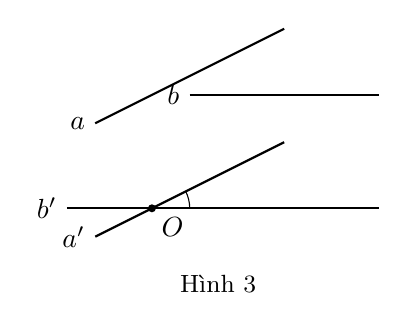
\begin{tikzpicture}[scale=1.2, >=stealth]
  % Line a
  \draw[thick] (0.5, 1.4) node[left] {$a$} -- (2.5, 2.4);
  % Line b
  \draw[thick] (1.5, 1.7) node[left] {$b$} -- (3.5, 1.7);
  
  % Line a' (parallel to a)
  \draw[thick] (0.5, 0.2) node[left] {$a'$} -- (2.5, 1.2);
  % Line b' (parallel to b)
  \draw[thick] (0.2, 0.5) node[left] {$b'$} -- (3.5, 0.5);
  
  % Intersection O
  \coordinate (O) at (1.1, 0.5);
  \fill (O) circle (1.2pt) node[below right] {$O$};
  
  % Angle arc
  \draw (1.1, 0.5) + (0:0.4) arc (0:26.6:0.4);
  
  \node[below] at (1.8, -0.1) {\small Hình 3};
\end{tikzpicture}
\end{center}
\end{minipage}

\vspace{0.4cm}

\noindent\textbf{\color{myblue}{2. Góc giữa đường thẳng và mặt phẳng}}\\
Cho đường thẳng $d$ và mặt phẳng $(P)$, ta có định nghĩa sau:
\begin{itemize}
    \item Nếu đường thẳng $d$ vuông góc với mặt phẳng $(P)$ thì góc giữa $d$ và $(P)$ bằng $90^\circ$.
    \item Nếu đường thẳng $d$ không vuông góc với mặt phẳng $(P)$ thì góc giữa đường thẳng $d$ và mặt phẳng $(P)$ là góc giữa $d$ và hình chiếu $d'$ của đường thẳng $d$ trên $(P)$ (Hình 4), kí hiệu $(d, (P))$.
\end{itemize}

\vspace{0.2cm}

\begin{center}
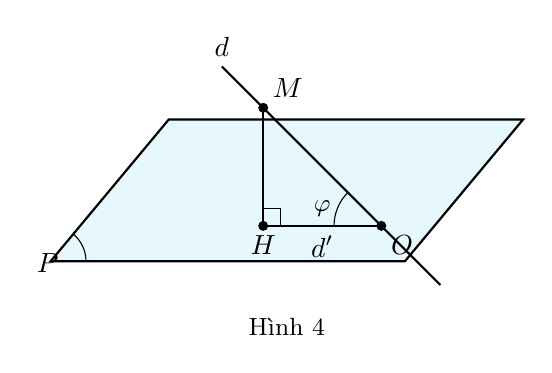
\begin{tikzpicture}[scale=1.5, >=stealth]
  % Plane P (filled with modern cyan!10)
  \fill[cyan!10] (0,0) -- (3,0) -- (4,1.2) -- (1,1.2) -- cycle;
  \draw[thick] (0,0) -- (3,0) -- (4,1.2) -- (1,1.2) -- cycle;
  \draw (0.3,0) arc (0:50:0.3);
  \node at (0.15,0.15) [below left] {$P$};
  
  % Coordinates
  \coordinate (O) at (2.8, 0.3);
  \coordinate (M) at (1.8, 1.3);
  \coordinate (H) at (1.8, 0.3);
  
  % Line d (above and below plane)
  \draw[thick] (1.45, 1.65) node[above] {$d$} -- (O);
  \draw[thick] (O) -- (3.3, -0.2);
  
  % Vertical line MH
  \draw[thick] (M) -- (H);
  
  % Projection line d' (HO)
  \draw[thick] (H) -- (O) node[midway, below] {$d'$};
  
  % Point labels
  \fill (M) circle (1.2pt) node[above right] {$M$};
  \fill (H) circle (1.2pt) node[below] {$H$};
  \fill (O) circle (1.2pt) node[below right] {$O$};
  
  % Right angle at H
  \draw (1.8, 0.45) -- (1.95, 0.45) -- (1.95, 0.3);
  
  % Angle phi at O
  \draw (2.8, 0.3) + (135:0.4) arc (135:180:0.4);
  \node at (2.3, 0.45) {\small $\varphi$};
  
  \node[below] at (2.0, -0.4) {\small Hình 4};
\end{tikzpicture}
\end{center}

\newpage

% Page 6: Dihedral Angle & Distances
\noindent\textbf{\textit{Nhận xét:}} Góc giữa đường thẳng và mặt phẳng có số đo từ $0^\circ$ đến $90^\circ$.\\

\noindent\textbf{\color{myblue}{3. Góc nhị diện}}\\
\begin{minipage}{0.55\textwidth}
\begin{itemize}
    \item Góc nhị diện là hình gồm hai nửa mặt phẳng có chung bờ; kí hiệu $[P, d, Q]$ hoặc $[M, d, N]$, trong đó $(P), (Q)$ là hai nửa mặt phẳng có chung bờ là đường thẳng $d$ và $M, N$ là các điểm lần lượt thuộc hai nửa mặt phẳng $(P), (Q)$ (Hình 5). Đường thẳng $d$ gọi là cạnh của góc nhị diện, mỗi nửa mặt phẳng $(P), (Q)$ gọi là một mặt của góc nhị diện.
    \item Cho góc nhị diện. Một góc có đỉnh thuộc cạnh của góc nhị diện, hai cạnh của góc đó lần lượt thuộc hai mặt nhị diện và cùng vuông góc với cạnh của góc nhị diện, được gọi là góc phẳng nhị diện của góc nhị diện đã cho.
    \item Số đo của một góc phẳng nhị diện được gọi là số đo của góc nhị diện đó.
    \item Nếu số đo góc phẳng nhị diện bằng $90^\circ$ thì góc nhị diện đó gọi là góc nhị diện vuông.
\end{itemize}
\textbf{\textit{Nhận xét:}} Góc nhị diện có số đo từ $0^\circ$ đến $180^\circ$.
\end{minipage}
\hfill
\begin{minipage}{0.4\textwidth}
\begin{center}
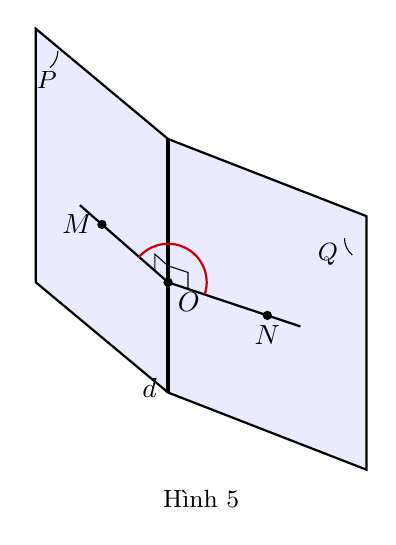
\begin{tikzpicture}[scale=1.4, >=stealth]
  % Plane P (left)
  \fill[blue!8] (0, -0.5) -- (-1.2, 0.5) -- (-1.2, 2.8) -- (0, 1.8) -- cycle;
  \draw[thick] (0, -0.5) -- (-1.2, 0.5) -- (-1.2, 2.8) -- (0, 1.8);
  
  % Plane Q (right)
  \fill[blue!8] (0, -0.5) -- (1.8, -1.2) -- (1.8, 1.1) -- (0, 1.8) -- cycle;
  \draw[thick] (0, -0.5) -- (1.8, -1.2) -- (1.8, 1.1) -- (0, 1.8);
  
  % Common edge d
  \draw[ultra thick] (0, -0.5) -- (0, 1.8) node[below left, pos=0.1] {$d$};
  
  % Coordinates
  \coordinate (O) at (0, 0.5);
  \coordinate (M) at (-0.6, 1.025);
  \coordinate (N) at (0.9, 0.2);
  
  % Lines OM and ON
  \draw[thick] (O) -- (-0.8, 1.2);
  \draw[thick] (O) -- (1.2, 0.1);
  
  % Points M, N, O
  \fill (O) circle (1.2pt) node[below right] {$O$};
  \fill (M) circle (1.2pt) node[left] {$M$};
  \fill (N) circle (1.2pt) node[below] {$N$};
  
  % Labels P and Q inside the planes
  \draw (-1.0, 2.6) arc (0:-50:0.2);
  \node at (-1.1, 2.5) [below] {\small $P$};
  
  \draw (1.6, 0.9) arc (180:230:0.2);
  \node at (1.45, 0.75) {\small $Q$};
  
  % Right angle symbols at O
  \draw (0, 0.65) -- (-0.12, 0.755) -- (-0.12, 0.605);
  \draw (0, 0.65) -- (0.18, 0.59) -- (0.18, 0.44);
  
  % Angle arc MON
  \draw[thick, myred] (0, 0.5) + (-18:0.35) arc (-18:140:0.35);
  
  \node[below] at (0.3, -1.3) {\small Hình 5};
\end{tikzpicture}
\end{center}
\end{minipage}

\vspace{0.4cm}

\noindent\textbf{\color{myblue}{\large III. KHOẢNG CÁCH TRONG KHÔNG GIAN}}\\
\noindent\textbf{\color{myblue}{1. Khoảng cách từ một điểm đến một đường thẳng}}\\
Khoảng cách từ điểm $M$ đến đường thẳng $\Delta$ là khoảng cách từ điểm $M$ đến hình chiếu vuông góc $H$ của $M$ trên $\Delta$, kí hiệu $d(M, \Delta)$.\\

\noindent\textbf{\color{myblue}{2. Khoảng cách từ một điểm đến một mặt phẳng}}\\
Khoảng cách từ điểm $M$ đến mặt phẳng $(P)$ là khoảng cách từ điểm $M$ đến hình chiếu vuông góc $H$ của $M$ trên $(P)$, kí hiệu $d(M, (P))$.\\

\noindent\textbf{\color{myblue}{3. Khoảng cách giữa hai đường thẳng song song}}\\
Khoảng cách giữa hai đường thẳng song song $\Delta$ và $\Delta'$ là khoảng cách từ một điểm bất kì thuộc đường thẳng này đến đường thẳng kia, kí hiệu $d(\Delta, \Delta')$.\\

\noindent\textbf{\color{myblue}{4. Khoảng cách giữa đường thẳng và mặt phẳng song song}}\\
Cho đường thẳng $\Delta$ song song với mặt phẳng $(P)$. Khoảng cách giữa đường thẳng $\Delta$ và mặt phẳng $(P)$ là khoảng cách từ một điểm bất kì thuộc đường thẳng $\Delta$ đến mặt phẳng $(P)$, kí hiệu $d(\Delta, (P))$.\\

\noindent\textbf{\color{myblue}{5. Khoảng cách giữa hai mặt phẳng song song}}\\
Khoảng cách giữa hai mặt phẳng song song $(P)$ và $(Q)$ là khoảng cách từ một điểm bất kì thuộc mặt phẳng này đến mặt phẳng kia, kí hiệu $d((P), (Q))$.\\

\noindent\textbf{\color{myblue}{6. Khoảng cách giữa hai đường thẳng chéo nhau}}\\
Cho hai đường thẳng $a, b$ chéo nhau.
\begin{itemize}
    \item Có và chỉ có một đường thẳng $c$ vừa vuông góc, vừa cắt cả hai đường thẳng $a, b$ gọi là đường vuông góc chung của hai đường thẳng đó.
    \item Đoạn thẳng có hai đầu mút là giao điểm của đường thẳng $c$ với hai đường thẳng $a, b$ gọi là đoạn vuông góc chung của hai đường thẳng đó.
    \item Độ dài đoạn vuông góc chung của hai đường thẳng $a, b$ gọi là khoảng cách giữa hai đường thẳng đó, kí hiệu $d(a, b)$.
\end{itemize}

\vspace{0.2cm}
\noindent\textbf{Nhận xét}

\newpage

% Page 7: Common Perpendiculars & Volume of Polyhedra
\begin{itemize}
    \item[\bluecheck] Gọi $(P)$ là mặt phẳng chứa $b$ và song song với $a$, hình chiếu của $a$ trên $(P)$ là $a'$, giao điểm của $a'$ và $b$ là $K$, hình chiếu của $K$ trên $a$ là $H$ (Hình 6). Khi đó $HK$ là đoạn vuông góc chung của $a$ và $b$. Ngoài ra, $d(a,b) = HK = d(a,(P))$.
\end{itemize}

\begin{center}
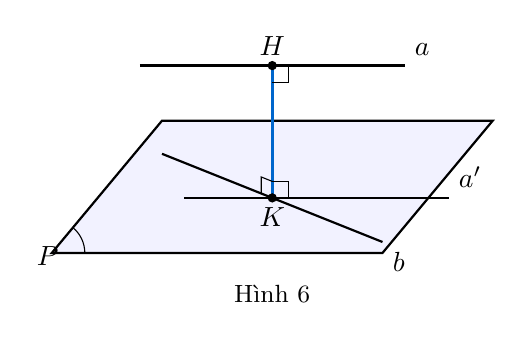
\begin{tikzpicture}[scale=1.4, >=stealth]
  % Plane P
  \fill[blue!5] (0,0) -- (3,0) -- (4,1.2) -- (1,1.2) -- cycle;
  \draw[thick] (0,0) -- (3,0) -- (4,1.2) -- (1,1.2) -- cycle;
  \draw (0.3,0) arc (0:50:0.3);
  \node at (0.15,0.15) [below left] {$P$};

  % Coordinates
  \coordinate (H) at (2.0, 1.7);
  \coordinate (K) at (2.0, 0.5);
  
  % Line a (above plane)
  \draw[thick] (0.8, 1.7) -- (3.2, 1.7) node[above right] {$a$};
  
  % Line a' (projection in plane)
  \draw[thick] (1.2, 0.5) -- (3.6, 0.5) node[above right] {$a'$};
  
  % Line b in plane, intersecting a' at K
  \draw[thick] (1.0, 0.9) -- (3.0, 0.1) node[below right] {$b$};
  
  % Vertical line HK (common perpendicular)
  \draw[very thick, myblue] (H) -- (K);
  
  % Point labels
  \fill (H) circle (1.2pt) node[above] {$H$};
  \fill (K) circle (1.2pt) node[below] {$K$};
  
  % Right angle at H (between a and HK)
  \draw (2.0, 1.55) -- (2.15, 1.55) -- (2.15, 1.7);
  
  % Right angle at K (between HK and a')
  \draw (2.0, 0.65) -- (2.15, 0.65) -- (2.15, 0.5);
  
  % 3D Right angle at K (between HK and b)
  \draw (2.0, 0.5) ++(-0.1, 0.04) -- ++(0, 0.15) -- ++(0.1, -0.04);
  
  \node[below] at (2.0, -0.2) {\small Hình 6};
\end{tikzpicture}
\end{center}

\begin{notebox}
\noindent\textbf{\color{myred}{\textit{*Trường hợp đặc biệt:}}}\\
\indent Trong trường hợp đặc biệt $a \perp b$, ta có thể xác định như sau: Gọi $(P)$ là mặt phẳng chứa $b$ và vuông góc với $a$, giao điểm của $a$ và $(P)$ là $H$, hình chiếu của $H$ trên $b$ là $K$ (Hình 7). Khi đó, $HK$ là đoạn vuông góc chung của $a$ và $b$.
\end{notebox}

\begin{center}
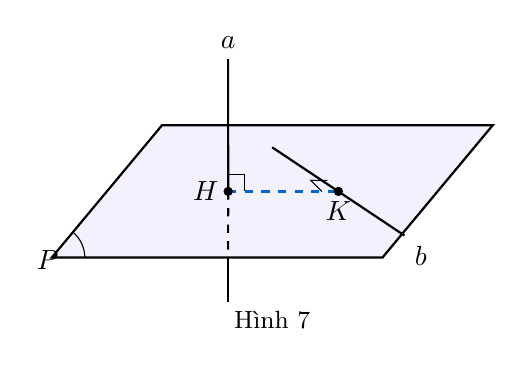
\begin{tikzpicture}[scale=1.4, >=stealth]
  % Plane P
  \fill[blue!5] (0,0) -- (3,0) -- (4,1.2) -- (1,1.2) -- cycle;
  \draw[thick] (0,0) -- (3,0) -- (4,1.2) -- (1,1.2) -- cycle;
  \draw (0.3,0) arc (0:50:0.3);
  \node at (0.15,0.15) [below left] {$P$};

  % Coordinates
  \coordinate (H) at (1.6, 0.6);
  \coordinate (K) at (2.6, 0.6);
  
  % Vertical line a
  \draw[thick] (H) -- (1.6, 1.8) node[above] {$a$};
  \draw[dashed, thick] (H) -- (1.6, 0);
  \draw[thick] (1.6, 0) -- (1.6, -0.4);
  
  % Line b in plane
  \draw[thick] (2.0, 1.0) -- (3.2, 0.2) node[below right] {$b$};
  
  % Dashed segment HK (common perpendicular)
  \draw[dashed, very thick, myblue] (H) -- (K);
  
  % Point labels
  \fill (H) circle (1.2pt) node[left] {$H$};
  \fill (K) circle (1.2pt) node[below] {$K$};
  
  % Right angle at H (between a and HK)
  \draw (1.6, 0.75) -- (1.75, 0.75) -- (1.75, 0.6);
  
  % Right angle at K (between HK and b)
  \draw (2.45, 0.6) -- (2.35, 0.7) -- (2.5, 0.7);
  
  \node[below] at (2.0, -0.4) {\small Hình 7};
\end{tikzpicture}
\end{center}

\vspace{0.4cm}

\noindent\textbf{\color{myblue}{\large IV. Thể tích của một khối đa diện}}\\
\begin{itemize}
    \item[\bluecheck] \textbf{Công thức tính thể tích của khối lăng trụ:} $V = S \cdot h$. \\
    Trong đó $V$, $S$, $h$ lần lượt là thể tích, diện tích đáy, chiều cao của khối lăng trụ.
    \item[\bluecheck] \textbf{Công thức tính thể tích của khối chóp:} $V = \frac{1}{3} S \cdot h$. \\
    Trong đó $V$, $S$, $h$ lần lượt là thể tích, diện tích đáy, chiều cao của khối chóp.
    \item[\bluecheck] \textbf{Công thức tính thể tích khối chóp cụt đều:} $V = \frac{1}{3} h \left(S_1 + \sqrt{S_1 S_2} + S_2\right)$.
    \item[\bluecheck] Trong đó $V$, $h$, $S_1$, $S_2$ lần lượt là thể tích, chiều cao, diện tích hai đáy của khối chóp cụt đều.
\end{itemize}

\end{document}
